\subsection{Tests}

To measure the scalability of Ethereum we prepared some tests to study
the maximal throughput and the size of the blockchain with different
configurations.
To study the scalability of one permission-less blockchain system such as
Ethereum one should prepare some tests using thousand of
nodes~\cite{bib:securityAndScalabilityPoW, bib:algorand}.
Since we do not dispose of so many resources we take inspiration from
Blockbench~\cite{blockbench}, which compares the performance and scalability
of Hyperledger\footnote{\url{https://www.hyperledger.org/}} and Ethereum in a
\emph{private} scenario, that is when
we take into consideration a limited number of authenticated nodes.

We tried to use the public available Blockbench
repository\footnote{\url{https://github.com/ooibc88/blockbench}}
but we did not manage to configure it, because of a lot of hard-coded
configuration variables and the lack of a well-written documentation.
Therefore we desisted and wrote our own system.


\subsubsection{Test Configuration}

To keep the configuration easy we opted for a classic master-slave logic.
The master, i.e. the initiator and coordinator of the tests, uses the ssh
protocol to run commands on the remote machines.
Similarly to~\cite{blockbench} we distinguish between the roles \emph{miner} and
\emph{client}. The nodes of the former type are accountable to generate new
blocks while the nodes of the latter type create and propagate transactions and
both verify the blocks\footnote{To reduce the number of test variables we
consider only full nodes}.
We can assign multiple roles to a single machine. In this case we run
\emph{one distinct geth instance} for each different role.
The coordinator copies the right genesis block in the test machines.



In each run of test we distinguish at least two phases:
\begin{enumerate*}
    \item the setup and
    \item the test itself.
\end{enumerate*}



\paragraph{Setup}
The setup consists in iterating on the test machines twice:
\begin{itemize}
\item In the first loop the required ethash data structures are generated,
\item In the second one a genesis file is used to initialize the
ethereum world state.
\end{itemize}


\paragraph{Ethash datastructure}

During the setup phase the nodes with the roles miner generate the
DAG and the cache for the first two epochs, while the clients generate only
the caches, because they are required only to validate blocks.
We generate the DAGs for the first two epochs, because ethash uses double
buffer of DAGs to grant a smooth switch between
epochs~\cite{bib:dagger-hashimoto}.



\paragraph{Genesis file}

The genesis file contains useful information to create (deterministically)
the genesis block and the initial state. It contains several parameters, such as
the maximum gas limit for the files, the difficulty and an initial allocation of
Ether for some accounts\footnote{This possibility has been used for the
so-called Initial Coin Offering (ICO) used by the Ethereum Foundation to obtain
fiat currency to finance the project.}. Clearly, each node of the network should
be initialized with the same genesis file. The genesis file for the main network
and the official Ethereum test networks are hard-coded. To create a new private
Ethereum network we use a new genesis file, in which we specify an arbitrary
networkid and nonce, so that the packets of different networks are simply
dropped as described in~\autoref{sec:ethereum-wire-protocol}.
In \autoref{} we show an extract of the genesis block we used.
Apart from the arbitrary values, that is the id and the nonce, other parameters
used in the tests require some justification, that we provide in the remainder
of this paragraph.

The \textbf{timestamp} of the genesis file, that corresponds to the one of the
genesis block, influences the difficulty of the first blocks, and transitively
of all the blocks.
Since, for time constraints, we want to run each test for few minutes we want
to avoid sudden decreases in the difficulty due to a too old timestamp.
Therefore, to prevent these unwanted changes in the difficulty value, during the
second loop of the setup phase, the initiator reads its timestamp and gives it
as parameter to the peers\footnote{Before starting the test all the
peers should be configured, therefore using the timestamp of the coordinator
does not assume fine-grained coordinated clocks.}

As already described in \autoref{sec:consensus:algorithm}, the
\textbf{difficulty} is an adaptive parameter  that determines how much effort
should be invested in the creation of a new block. In our tests we used the same
hardware and same operating system in all nodes and for all miners (we
deliberately used only one thread for mining). Therefore to find a suitable
start value for the difficulty for the different configurations we ran a
simulation with one, two, four and eight miners for 24 hours.
\autoref{fig:start_difficulty_raw} shows how the difficulty changed with the
different number of miners. We can notice that in our homogeneous system the
final values of difficulties have a quasi linear dependency with the number of
miners. For the test we took as initial value the median of the last $100$
blocks.
\begin{figure}
    \begin{center}
        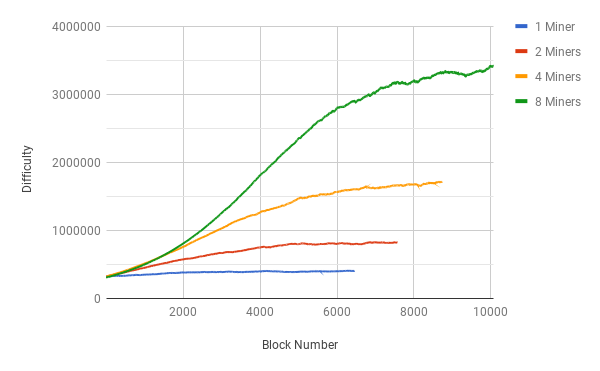
\includegraphics[width=0.8\textwidth]{./res/img/start_difficulty_all.png}
        \caption{The growth of the difficulty in the 24 hour run.}
        \label{fig:start_difficulty_raw}
    \end{center}
\end{figure}

The \textbf{gas limit} in the genesis block determines the gas limit of the
first block. The gas limit of the subsequent blocks can be determined freely by
the miners but must be contained in a range obtained by summing and subtracting
to the gas limit a portion of itself~\cite{wood2018ethereum}.
Thus, in a relative brief simulation the
initial value is foundamental. Due to the considerations of
\autoref{sec:background}, we decided to use a large value for the gas limit,
i.e. $500 \cdot 21000$, that corresponds to the gas to execute $500$
transactions without execution of code.



\paragraph{Maximal Throughput Test}
We wanted to measure the maximal throughput with different number of miners,
to prove or disprove that the system can scale out.

In our tests we keep the number of clients and the number of emitted 
transactions constant, indeed we used $16$ clients (2 clients per machine) that 
propagate a new  transaction each $50$ ms.
